% ДЗ на 06.12.2022
% Михедов Константин БИБ224

% Статья на А4, 12 кегель
\documentclass[a4paper,12pt]{article}

% Поиск по скомпилированному PDF
\usepackage{cmap}
% Кодировка выходного текста
\usepackage[T2A]{fontenc}
% Кодировка исходного текста
\usepackage[utf8]{inputenc}
% Поддержка необходимых языков
\usepackage[english,russian]{babel}

% Поддержка изображений
\usepackage{graphicx}
% Путь до внешних изображений
\graphicspath{ {./figures/}}

% Умная запятая
\usepackage{icomma}

% Ссылки на электронные ресурсы
\usepackage{hyperref}
% Настройка внешнего вида ссылок
\hypersetup{
  % Отключить прямоугольную рамку
  pdfborder={0 0 0},
  % Включить цветные ссылки
  colorlinks=true,
  % Цвет для ссылок на веб-ресурсы
  urlcolor=blue,
  % Цвет внутренних ссылок
  linkcolor=black
}

% Дополнительная математика
\usepackage{amsmath,amsfonts,amssymb,amsthm,mathtools}
% Показывать номера только у тех выржений, на которые кто-то ссылается
\mathtoolsset{showonlyrefs=true}

% Дополнительные символы
\usepackage{mathbbol}

% Правильное оформление
% Настройка отступов
\usepackage[left=2cm,right=1cm,top=2cm,bottom=2cm]{geometry}
% Настройка шрифта
\usepackage{fontspec}
\setmainfont{Times New Roman}
% Настройка межстрочных интервалов
\usepackage{setspace}
\onehalfspacing
% и межабзацных
\usepackage{parskip}
\setlength{\parindent}{1.25cm} 

% Красная строка
\usepackage{indentfirst}
\setlength{\parindent}{1.25cm} 

% Корректное положение рисунков?
\usepackage{float}

% Расположение блоков относительно текста
\usepackage{wrapfig}

\begin{document}
    \paragraph{Работу выполнил} Михедов Константин Константинович БИБ224

    \section*{Задача №1}

    \paragraph{Условие} Пассажир бежит и вскакивает на движущуюся со скорость
    2 км/ч в одном направлении с ним открытую платформу поезда. С какой скоростью
    будет двигаться открытая платформа поезда, если вес пассажира 588 Н,
    скорость пассажира 9 км/ч, вес платформы 784 Н? С какой скоростью будет
    двигаться открытая платформа, если бы пассажир бежал ей навстречу?

    \begin{figure}[H]
        \minipage{0.2\textwidth}
            \begin{tabular}{p{0.8\textwidth} |}
                \textbf{Дано} \\
                \hline
                $v_t = 2$ км/ч \\
                $v_p = 9$ км/ч \\
                $P_p = 588$ Н \\
                $P_t = 784$ Н \\
                \hline
                $v_1 = $? $v_2 = $?
            \end{tabular}
        \endminipage
        \minipage{0.79\textwidth}
            \textbf{Решение}

            В данном случае действие силы трения считаем равным $0$ $\Rightarrow$ можем
            использовать закон сохранения импульcа (далее ЗСИ)

            По условию возможны два случая: пассажир и платформа движутся в одном направлении
            (рис. \ref{img:t1:1}) или пассажир и платформа движутся в противоположных направлениях
            (рис. \ref{img:t1:2})
        \endminipage
    \end{figure}
    \begin{figure}[H]
        \centering
        \minipage{0.4\textwidth}
            \centering
            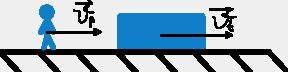
\includegraphics[scale=1.3]{01_01}
            \caption{первый случай}
            \label{img:t1:1}
        \endminipage
        \minipage{0.4\textwidth}
            \centering
            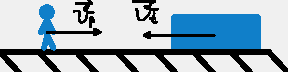
\includegraphics[scale=1.3]{01_02}
            \caption{второй случай}
            \label{img:t1:2}
        \endminipage
    \end{figure}

    Пусть ось X будет сонаправлена с вектором $\vec{v_p}$, а ось Y - перпендикулярна ему и направелна вверх,
    тогда видно, что в обоих случаях $v_{py} = v_{ty} = 0$ $\Rightarrow$ для заданных тех вес численно
    равен силе тяжести: $|\vec{P}| = m|\vec{g}|$ $\Leftrightarrow$ $m = \frac{|\vec{P}|}{|\vec{g}|}$. Отсюда
    $m_p = P_p / g$ и $m_t = P_t / g$

    Запишем ЗСИ в векторной форме: $\sum{\vec{p}_{\text{до}}} = \sum{\vec{p}_{\text{после}}}$
    $\Leftrightarrow$ $m_p\vec{v}_p + m_t\vec{v}_t = (m_p + m_v)\vec{v}_r$

    Рассмотрим первый случай в проекциях на ОХ:
    \begin{multline}
        m_pv_p + m_tv_t = (m_p + m_t)v_r \Leftrightarrow \\ \Leftrightarrow
        v_t = \frac{m_pv_p + m_tv_t}{m_p + m_t} 
        = \frac{\frac{P_p}{g}v_p + \frac{P_t}{g}v_t}{\frac{P_p + P_t}{g}} =
        \frac{P_pv_p + P_tv_t}{P_p + P_t} = \\ =
        \frac{588H\cdot 9\text{км/ч} + 784H\cdot 2\text{км/ч}}{588H + 784H}
        = 5\text{км/ч}
    \end{multline}

    И второй случай также в проекциях на OX:
    \begin{multline}
        m_pv_p - m_tv_t = (m_p + m_t)v_r \Leftrightarrow \\ \Leftrightarrow
        v_t = \frac{m_pv_p - m_tv_t}{m_p + m_t} 
        = \frac{\frac{P_p}{g}v_p - \frac{P_t}{g}v_t}{\frac{P_p + P_t}{g}} =
        \frac{P_pv_p - P_tv_t}{P_p + P_t} = \\ =
        \frac{588H\cdot 9\text{км/ч} - 784H\cdot 2\text{км/ч}}{588H + 784H}
        = \frac{19}{7}\text{км/ч} \approx 2.7\text{км/ч}
    \end{multline}

    \begin{flushright}
        \textbf{Ответ:} 5 км/ч и 2.7 км/ч
    \end{flushright}

    \section*{Задача №2}

    \paragraph{Условие} На скамье Жуковского стоит человек и держит в руках стержень длиной
    2.4 м и массов 8 кг, расположенный вертикально по оси вращения скамейки. Скамья с человеком
    вращается с частотой 1 Гц. С какой частотой будет вращаться скамья с человеком, если он
    повернет стержень в горизонтальное положение? Суммарный момент инерции человека и
    скамьи равен 6 кг$\cdot$м$^2$

    \begin{figure}[H]
        \minipage{0.2\textwidth}
            \begin{tabular}{p{0.8\textwidth} |}
                \textbf{Дано} \\
                \hline
                $l = 2$м \\
                $m = 8$кг \\
                $f_1 = 1$Гц \\
                $J_{sum} = 6$кг$\cdot$м$^2$ \\
                \hline
                $f_2 = $?
            \end{tabular}
        \endminipage
        \minipage{0.79\textwidth}
            \textbf{Решение}

            \begin{figure}[H]
                \centering
                \minipage{0.4\textwidth}
                    \centering
                    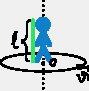
\includegraphics[scale=1.5]{01_03}
                    \caption{было}
                    \label{img:t2:1}
                \endminipage
                \minipage{0.4\textwidth}
                    \centering
                    
\includegraphics[scale=1.5]{01_04}
                    \caption{стало}
                    \label{img:t2:2}
                \endminipage
            \end{figure}
        \endminipage
    \end{figure}

    По закону сохранения момента импульса (далее ЗСМИ) $\vec{L_1} = \vec{L_2}$, где
    $\vec{L} = J\vec{\omega}$

    Время одного оборота скамьи Жуковского $T = f^{-1} = \frac{2\pi}{\omega}$
    $\Leftrightarrow$ $\omega = 2\pi f$

    Рассмотрим общий момент инерции для первой системы тел (рис. \ref{img:t2:1}):
    $J_1 = J_{sum} + J_{l1}$. Так как стержень в данном случае расположен вертикально,
    можем считать его момент инерции равным нулю: $J_{l1} = 0$ $\Rightarrow$ $J_1 = J_{sum} + J_{l1} = J_{sum}$

    Теперт рассмотрим второй случай (рис. \ref{img:t2:2}): $J_2 = J_{sum} + J_{l2}$. Здесь стержень
    уже влияет на общий момент инерции $\Rightarrow$ $J_{l2} \neq 0$

    \begin{wrapfigure}{r}{0.25\textwidth}
        \centering
        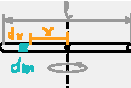
\includegraphics[width=0.25\textwidth]{01_05}
    \end{wrapfigure}

    Теперь необходимо найти $J_{l2}$. Видно, что $dm = \frac{m}{l}dx$

    Известно, что $J = mr^2$, в нашем случае $J_{l2} = mx^2$. Продеффиренцируем это
    выражение: $dJ_{l2} = d(x^2m) = x^2dm = x^2 \frac{m}{l}dx$

    Проинтегрируем полученное выражение:

    \begin{equation}
        J_{l2} = \int_{-l/2}^{l/2}dJ_{l2} = \int_{-l/2}^{l/2}\frac{x^2m}{l}dx =
        \frac{mx^3}{3l}|_{-l/2}^{l/2} = \frac{ml^3}{3l \cdot 8} - \frac{-ml^3}{3l\cdot 8}
        = 2\frac{ml^2}{24} = \frac{ml^2}{12}
    \end{equation}

    Тогда $J_2 = J_{sum} + J_{l2} = J_{sum} + \frac{ml^2}{12}$. Подставим полученные значения в ЗСМИ:
    \begin{multline}
        L_{z1} = L_{z2} \Leftrightarrow
        J_1\omega_{z1} = J_2\omega_{z2} \Leftrightarrow
        2\pi J_{sum}f_1 = (J_{sum} + \frac{ml^2}{12})\cdot 2\pi f_2 \Leftrightarrow \\
        \Leftrightarrow
        f_2 = \frac{2\pi J_{sum}f_1}{2\pi(J_{sum} + \frac{ml^2}{12})} =
        \frac{J_{sum}f_1}{J_{sum} + ml^2/12} = \\
        = \frac{6\text{кг}\cdot\text{м}^2 \cdot 1\text{Гц}}{6\text{кг}\cdot\text{м}^2 + 8\text{кг} (2\text{м})^2/12}
        = \frac{9}{13}\text{Гц} \approx 0.69 \text{Гц}
    \end{multline}

    \begin{flushright}
        \textbf{Ответ:} 0.69 Гц
    \end{flushright}

    \section*{Задача №3}

    \paragraph{Условие} Цилиндры: сплошной алюминиевый и полый свинцовый одинакового радиуса 6 см
    и одинакового веса 4.5Н, окрашенные одинаково скатываются без скольжения по наклонной
    плоскости. Как наблюдая поступательные скорости цилиндров у подножия наклонной
    плоскости различить их? Нати моменты инерции этих цилиндров, время скатывани без
    скольжения по наклонной плоскости, если дано, что высота наклонной плоскости 0.5м, угол наклона
    плоскости 30, а начальная скорость каждого цилиндра равна нулю.

    \begin{figure}[H]
        \minipage{0.3\textwidth}
            \begin{tabular}{p{0.55\textwidth} | p{0.25\textwidth} |}
                \textbf{Дано} & \textbf{СИ} \\
                \hline
                $r_1 = r_2 = 6$см & 6$\cdot10^{-2}$м \\
                $P_1 = P_2 = 4.5$Н &\\
                $h = 0.5$м & \\
                $\alpha = 30^{\circ}$ &\\
                \hline
                \multicolumn{2}{c|}{
                    $v_1 = $ ? $v_2 = $ ?
                    $J_1 = $ ?
                } \\
                \multicolumn{2}{c |}{
                    $J_2 = $ ?
                    $t_1 = $ ? $t_2 = $ ?
                }
            \end{tabular}

            \begin{figure}[H]
                \centering
                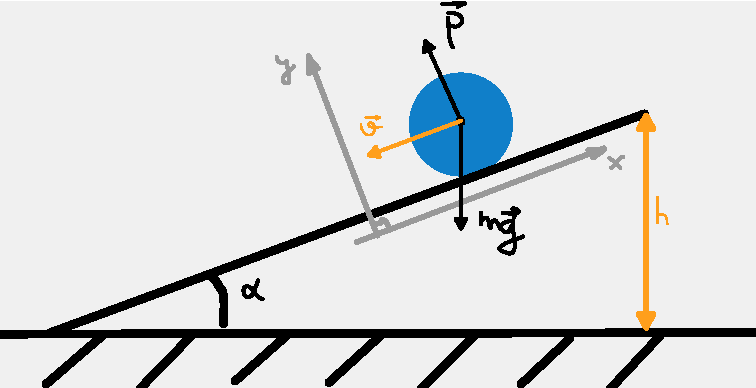
\includegraphics[width=0.9\textwidth]{01_06}
                \caption{сплошной цилиндр}
                \label{img:t3:1}
            \end{figure}
        \endminipage
        \minipage{0.7\textwidth}
            \textbf{Решение}

            Длина наклонной плоскость $l = \frac{h}{\sin\alpha}$. Пусть $r = r_1 = r_2$, а
            $P = P_1 = P_2$, $a$ - высота первого цилиндра, $b$ - высота второго
            и $J_1$ - момент инерции сплошного (алюминиевого) цилиндра, а
            $J_2$ - полого (свинцового), тогда $J_1 = 0.5m_1r^2$, а $J_2 = m_2r^2$
            \begin{multline}
                J_1 = \int_0^{r_1} \rho_1 r^2 dV = \int_0^{r_1} \rho_1 r^2 d(2\pi r^2 a)= \\ =
                \int_0^{r_1} 2\pi r^3 a\rho_1 dr = 2\pi a\rho_1\int_0^{r_1} r^3dr =\\
                = \frac{2\pi a r_1^4}{4} \cdot \rho_1 = \frac{2\pi a r_1^4}{4} \cdot
                \frac{m_1}{\pi r^2 a} = \frac{m_1r_1^2}{2} = \frac{m_1r^2}{2}
            \end{multline}
            \begin{equation}
                J_2 = \int_0^{m_2} r^2dm = m_2r^2
            \end{equation}
        \endminipage
    \end{figure}

    Распишем второй закон Ньютона в векторном виде:
    $\vec{P} + m\vec{g} = m\vec{a}$ (где $m$ или $m_1$, или $m_2$). Тогда для первого тела
    в проекциях на ОУ: $P - m_1g/\cos\alpha = 0$ $\Leftrightarrow$ $m_1 = \frac{P\cos\alpha}{g}$,
    а для
    второго тела в проекциях на ОУ: $m_2 = \frac{P\cos\alpha}{g}$.
    Получается, что $m = m_1 = m_2 = \frac{P\cos \alpha}{g}$

    Так как цилиндры учавствуют и в поступательном, и во вращательном движении, то
    полная механическая энергия в конце движения
    $W = W_{\text{п}} + W_{\text{в}} = \frac{mv^2}{2} + \frac{J\omega^2}{2} = \frac{mv^2 + J\omega^2}{2}$.
    Действие силы трения равно нулю по условию, $\Rightarrow$ $W = W_p = mgh$, то есть для
    первого цилиндра:
    \begin{multline}
        \frac{mv_1^2 + J\omega_1^2}{2} = mgh \Leftrightarrow
        mv_1^2 + J_1\omega_1^2 = 2mgh \Leftrightarrow
        mv_1^2 + J_1(\frac{v_1}{r})^2 = 2mgh \Leftrightarrow \\
        \Leftrightarrow
        v_1^2 (m + \frac{J_1}{r^2}) = 2mgh \Leftrightarrow
        v_1^2 \cdot \frac{mr^2 + J_1}{r^2} = 2mgh \Leftrightarrow
        v_1^2 = \frac{2mghr^2}{mr^2 + J_1} \Leftrightarrow \\
        \Leftrightarrow v_1 = \sqrt{
            \frac{2mghr^2}{mr^2 + \frac{mr^2}{2}}
        } = \sqrt{
            \frac{4mghr^2}{3mr^2}
        } = \sqrt{
            \frac{4gh}{3}
        }
    \end{multline}

    Аналогично для полого цилиндра:
    \begin{equation}
        v_2 = \sqrt{
            \frac{2mghr^2}{mr^2 + J_2}
        } = \sqrt{
            \frac{2mghr^2}{mr^2 + mr^2}
        } = \sqrt{
            gh
        }
    \end{equation}

    Так как начальная скорость равна 0, то $s(t) = \frac{at^2}{2} = \frac{vt}{2}$ $\Rightarrow$
    $t_1 = \frac{2l}{v_1}$ и $t_2 = \frac{2l}{v_2}$

    Итого, вычислим все значения (\textbf{Ответ}):
    \begin{equation}
        \begin{aligned}
            &J_1 = \frac{mr^2}{2} = \frac{Pr^2\cos\alpha}{2g} =  7\cdot 10^{-4} \text{кг}\cdot\text{м}^2 & 
            &J_2 = mr^2 = 2J_1 = 1.4 \cdot 10^{-3} \text{кг}\cdot\text{м}^2 \\
            &v_1 = \sqrt{
                \frac{4gh}{3}
            } = 2.6 \text{м/с}  &
            &v_2 = \sqrt{gh} = 2.2 \text{м/с} \\
            &t_1 = \frac{2l}{v_1} = \frac{2h}{v_1\sin\alpha} = 0.8 \text{с} &
            &t_2 = \frac{2l}{v_2} = \frac{2h}{v_2\sin\alpha} = 0.9 \text{с}
        \end{aligned}
    \end{equation}
\end{document}
